Fourier Volume Registration within the context of a 3D reconstruction procedure requires two frames of 3D data. These two frames may be input as any 3D representation: mesh, volume, point-cloud, SDF or in a compressed format (e.g. Octree). However, the input must be converted to a 3D signal or volume representation prior to phase correlation. Moreover, the size of the volume should be cubic and the data should be scaled to fit. If the two frames are scaled un-evenly then the method must also be registered against scale. This section details some of these issues and others within the context of video sensor input from sensors.  \\
 

\subsubsection{Camera Translation}
\label{sec:PCForSLAM}
To describe camera translation, let us say a camera produces 3D scans of a scene from a particular pose. This may be performed implicitly (in the case of stereo or monocular depth estimation procedures) or explicitly (through the use of sensors, i.e. Microsoft Kinect, Asus Xtion Pro Live) and the scans may be normalized into 3D volume frames. If the camera captured frame 1, then moved 20 units to the left, before capturing frame 2, visualizing these frames in conjunction with each-other, it would appear the data was shifted to the right by $20$ units ($20\theta$ if the resolution of the 3D volume differs by a scale of $\theta$). If the volumes were to be registered (assuming no error), it would be found that the data from frame 1 to frame 2 had been translated by $T_{frame-1,frame-2} = [20,0,0]^T$, which can be performed using the translation matrix in equation \ref{eqn:TransRegMatrix}.

\begin{equation} \label{eqn:TransRegMatrix}
\left[
\begin{array}{cccc}
1 & 0 & 0 & 20 \\
0 & 1 & 0 & 0 \\
0 & 0 & 1 & 0 \\
0 & 0 & 0 & 1 \\
\end{array}
\right]
\end{equation}

The volume data has shifted in the opposite direction. Therefore to register the data, frame 1 may be transformed by the matrix in equation \ref{eqn:TransRegMatrix} to align it with frame 2. Conversely, the camera pose may be updated by adding $T_{frame-1,frame-2} \times -1$ to the camera's location.  \\

Generalizing this, we define a volume $V_1$ captured as the first frame and a second volume $V_2$ which is captured after moving the camera in a particular direction (up, down, left, right, forward or backward) scaled by a magnitude (a vector). The translation from $V_1$ to $V_2$, $(x,y,z)$ can easily be recovered via phase correlation. As described, the camera pose may be updated by $-1 \times (x,y,z) = (-x,-y,-z)$. \\

Here we step into the detail of phase correlation with deeper insight than the superficial introduction in section \ref{Sec:SuperficialPCSection} and with a focus on 3D data and pose estimation. Firstly, we define the correlation measure process. Correlation in the context of signal processing measures signal shape similarity between two signals. \\

In this measure, large correlation values signify a greater similarity in terms of shape, while a smaller value signifies the signals have very different shapes. Note, large negative values signify the shapes may be similar but mirrored. Following the doctrine of DSP, that all signals, no matter what dimension may be processed similarly with similar operations and measures, this technique can be applied to measure similarities between volumes.  \\

The measure of correlation between $V_1$ and $V_2$ can be found by shifting $V_1$ and $V_2$'s mean values to zero. By doing this, the mean value cannot affect the correlation measure. For example, if the first frame was captured in low light and the second in a brighter light. The resulting values for frame 2 may look like those from frame 1 in terms of values fluctuating about a mean, however the change in lighting may affect the voxel values by increasing them by a uniform value or scaling them by some scalar. Therefore, by subtracting the mean we place the signals in states where by their shape, rather than their raw values may be compared. The procedure can then be completed by summing the element-wise multiplication of $V_1$ by $V_2$. When $V_1$ has a positive voxel value (a voxel value above the mean) as does $V_2$'s corresponding voxel in the same position, the multiplication value is positive, and this is summed into the correlation measure. This is the same situation if both voxel values were negative (both below the mean). On the other hand, if one voxel value was positive and the other negative, the correlation measure would be rectified accordingly. Equation \ref{eqn:CorrelationEquation} computes this correlation measure. 

\begin{equation} \label{eqn:CorrelationEquation}
\sum_{z=0}^{N}\sum_{y=0}^{N}\sum_{x=0}^{N}(V_1(x,y,z)-avg(V_1)) \times (V_2(x,y,z)-avg(V_2))
\end{equation}

As mentioned, correlation may be used to measure the similarity between two volumes' shapes. In the context of registration for 3D reconstruction algorithms, it can be used to measure the accuracy of a registration. This again uses $V_1$ as frame 1 and $V_2$ as frame 2, given a supposed transform $T_{est}$ to register $V_1$ to $V_2$. The measure of registration may be defined as $correlate(T_{est}(V_1), V_2)$. The measure may be used to compare two registrations, possibly to select the better registration in terms of correlation measure. The two frames may be captured under different lighting conditions and the correlation measure can still be used to select the best transform. \\


Within the framework of measuring camera pose, the cross-correlation algorithm may be used to measure the correlation values for each possible camera movement, and define the camera location as the location with the largest correlation value. This algorithm is shown in listing \ref{algorithm:CrossCorrelationAlgorithm}.

\begin{figure}
\begin{lstlisting}[language=c++,caption=Cross-Correlation based camera location estimation,label=algorithm:CrossCorrelationAlgorithm,mathescape,basicstyle=\ttfamily]
$V_1$ = CaptureFrame();
//shift camera
$V_2$ = CaptureFrame();
$highest-correlation$ = $infty $;
camera-location = $[0,0,0]$;
for($z$ in $[0,N]$){
  for($y$ in $[0,N]$){
    for($x$ in $[0,N]$){
      $V_{temp}$ = translate(V_1, x, y, z);
	  $tempMeasure$ = correlate($V_{temp}$, $V_2$);
	  if($tempMeasure$ > $highest-correlation$){
	    $highest-correlation$ = $tempMeasure$;
		$camera-location$ = $[-x,-y,-z]$;
	  }		
	}
  }
}
\end{lstlisting}
\end{figure}

Cross correlation is typically used in signal processing to compute the best alignment for two signals. In this context it has been used to compute the best camera location change, notice in the algorithm the $camera-location$ variable is set to be the inverse of the translation amount being tested ($[-x,-y,-z]$). Again this is because when the optimal translation value aligning frame 1 to frame 2 is defined as vector $v$, then the camera location change is equivalent to the inverse. The cross-correlation function in this context may be thought of as an exhaustive optimization procedure which optimizes the camera location change (equation \ref{eqn:CrossCorrelationEquation11}) in terms of the correlation function.  \\

\begin{equation} \label{eqn:CrossCorrelationEquation11}
correlate(translate(V_1, x,y,z), V_2)
\end{equation}

The range of camera location vectors to test is dependent on the dimensions of the raw 3D input data. If the data is scaled to fit an $N^3$ space, as is a requirement when using Fourier based techniques, the camera location values along the x, y and z axis would range between 0 and $N$. To compute the optimal camera location change using the phase correlation method would therefore have complexity $N^3$. There are $N^3$ values to test, and the correlation function must be called for each iteration with a complexity also equivalent to $N^3$, $N^3 \times N^3 = N^6$. This is significantly complex, even for smaller volume sizes. Note that the smaller the volume size, the faster the algorithm, however the more quantized the original data is. The more the input data is quantized, the more the camera location change estimates will be restricted in terms of precision. Accuracy will also be affected as quantization introduces unwanted effects of its own. The answer is to use the properties of the Fourier transform to speed up the process.  \\

The 3D Fourier transform transforms a volume from the 3D spatial domain into the 3D frequency domain (see Figure \ref{fig:FrequencyDomainExample}). The frequency domain is a complex valued volume made up of sinusoids. Each voxel in the frequency domain represents the magnitude, phase and direction of a wave. The importance of these properties for computing camera pose will be discussed upcoming sections. An efficient software implementation of the Fourier transform, named the Fast Fourier Transform (FFT), can compute the frequency domain given N-dimensional data. \\


\begin{figure}[!htb]
\centering
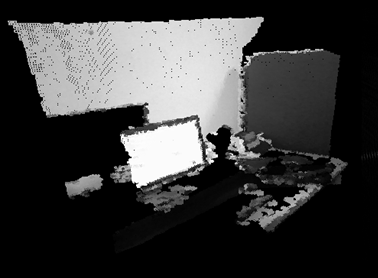
\includegraphics[width=6cm]{images/methodology/FVR/capFrameOriginal}
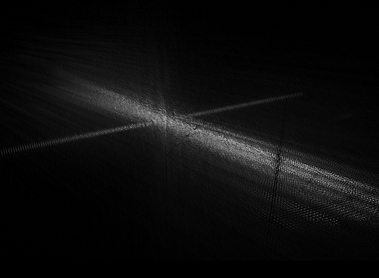
\includegraphics[width=6cm]{images/methodology/FVR/capFrameMagFFT}
\caption{Left: Captured 3D frame, Right: Magnitude values in the frequency domain of the captured 3D frame}
\label{fig:FrequencyDomainExample}
\end{figure}
 

Exploiting the properties of the FFT and the frequency domain, cross-correlation may be carried out efficiently to compute the optimal camera location change between frames. In the 2D approach, this algorithm is named phase correlation and is a popular approach in 2D image processing to align two images. Applied to two 3D frames captured by sensors (or partially generated via software) it may also be used to register the frames for 3D reconstruction as well as compute the translation part of the camera pose change for SLAM algorithms. This procedure is defined here as a function named $PhaseCorrelation$ (Eq. \ref{eqn:PC_basic}). This function takes two frames (3D volumes) as input and returns the best translation alignment between them in terms of maximizing correlation.  \\

\begin{equation} \label{eqn:PC_basic}
T(x, y, z) = PhaseCorrelation(V_x, V_y)
\end{equation}

The $PhaseCorrelation$ consists of four steps. In the first step the two captured 3D frames $V_1$ and $V_2$ are transformed into the frequency domain using the Fast Fourier Transform. This computes two new volumes $F_{1_{x,y,z}} = FFT(V_1)$ and $F_{2_{x,y,z}} = FFT(V_2)$. Applying the Fourier Shift Theorem to the context of camera pose estimation, if frames $V_1$ and $V_2$ are separated by some camera translation, then $F_{1_{x,y,z}}$ and $F_{2_{x,y,z}}$ will have phase values shifted relative to each-other. The normalized cross power spectrum (equation \ref{eqn:PHCOR_eq}) of the two complex valued Fourier spaces may then be used to find the camera translation change. The normalized cross power spectrum of $F_{1_{x,y,z}}$ and $F_{2_{x,y,z}}$ is another complex valued volume of the same size. \\

\begin{equation} \label{eqn:PHCOR_eq}
F_{3_{x,y,z}} = \frac{F_{1_{x,y,z}} \circ F_{2_{x,y,z}}^*}{ | F_{1_{x,y,z}} \circ F_{2_{x,y,z}}^* | }
\end{equation}

In equation \ref{eqn:PHCOR_eq}, $\circ$ is an element-wise multiplication and $|x|$ is the magnitude function or absolute value function. The Inverse Fast Fourier Transform ($IFFT$, $FFT^{-1}$) may then be used on the output of the normalized cross power spectrum volume to produce a phase correlation surface. The peak value on the phase correlation surface represents the optimal value of the correlation function applied to the two original real valued 3D frames. Therefore, the $PhaseCorrelation$ procedure is equivalent to the cross-correlation procedure, but rather than being complexity $N^6$, phase correlation reduces the complexity to approximately $6N^3 \times Log(N)$. \\


Due to the nature of camera capture, if the camera is translated by some vector before the capture of the next frame then the first frame contains data which the second frame does not. Conversely, the second frame will capture some other data which is not present in the first frame (unless the camera was not moved). The parts of the 3D frames which do not overlap cause noise on the phase correlation surface. This makes it more difficult to decipher the location of the peak. There may be several peaks to choose from, or no clear peak. The nature of computing the Discrete Fourier Transform affects peak estimation. The Discrete Fourier Transform assumes the output Fourier space is an infinitely repeating signal. The cross-correlation procedure on the other hand does not assume this, so therefore the phase correlation surface may be affected. The solution adopted by many is to filter the volumes prior to transforming into the frequency domain. This can be done using a Hanning window function (equation \ref{eqn:HanningFunction}). This function can be used to filter edge effects prior to computing the Fourier transform which helps to reduce noise on the phase correlation surface. \\

\begin{equation} \label{eqn:HanningFunction}
Hanning(x) = \frac{1}{2}(1 - cos\left(\frac{2\pi x}{\frac{N}{2} - 1}\right)
\end{equation}

Noise on the phase correlation surface may also be present if other types of transforms are present. In this case, the true camera translation may be lost. Therefore, camera pose/rotation must be computed prior to computing the camera translation. Other artefacts which may produce noise on the phase correlation surface include moving objects. If an object is present in one scene and not the other, it will cause some noise to be present in the phase correlation surface, making finding the peak more difficult but not impossible. Alternatively if there is an object whose location is changed between frames, the same thing may happen. The phase correlation procedure should already be robust to these artefacts but filtering approaches may also prove useful in selecting the correct peak which optimizes the translation used to register the 3D camera frames. \\

\subsubsection{Camera Rotation and Zooming}
\label{Sec:RoteZoomingSection}

SLAM and 3D reconstruction algorithms must compute both the camera location changes and camera pose. SLAM must compute the pose to track the camera, 3D reconstruction methods may simply register the data for integration or compute the camera pose prior to alignment and integration. Computing the pose involves estimating the camera's post change (rotation) from one frame to another. This may take the form of a $4 \times 4$ rotation matrix or the explicit magnitudes of rotation for each axis in a pre-determined order. These two formats may be converted between each other. The pose may also be represented by three axes (three orthogonal vectors) which represent the coordinate space of the camera. \\

Another transform often not covered in the 3D reconstruction literature is that of scale. Given a single camera moving in a 3D space, scale is of no concern. However, if frames are zoomed or data is computed across sensors, scale factors may be unknown. For example, if an RGB-D image is captured as frame 1 and a second is captured as frame 2, but frame 2 is zoomed (scaled) prior to projection, then the data may still be registered if scale can also be recovered. Alternatively, if frame 2 is captured by another sensor or software system and is projected at a different scale, then this scale should also be recovered. The recovery of scale could be considered most important in the case of monocular 3D reconstruction. Here, the fundamental matrix may be used to calibrate camera frames. Once calibrated, stereo methods may be used to extract dense depth information for each frame. The problem with this technique is that depth is relative, but not to scale, across multiple frames. If the scale can also be recovered during the camera pose estimation procedure it would eliminate the need for more advanced methods of optimization. \\ 

Phase correlation alone cannot register against camera rotation. An important part of SLAM is the ability to recover 3D camera pose, and a fundamental part of 3D reconstruction is to align dense depth data against as many camera movements as possible. Therefore, I propose using an extension of the popular rotation and scale recovery procedure from 2D registration research to perform camera rotation change estimation as well as align frames which have been zoomed or scaled to fit the volumetric space. \\

Using the rotation and scale recovery technique, which is comprised of a few spatial transformations and a phase correlation, a single axis of rotation may be recovered. The axis chosen is integrated into the spatial transformation part of the procedure. Since most scenes would be captured by moving around a room and rotating the camera to look at the areas within the scene directly around the user and camera, we have designated the y-axis of rotation as the most important axis to recover. Additionally, vehicles (with dash mounted cameras) and robots typically keep the camera steady and perform movements and rotations about the y-axis. The application of this rotation and scale recovery technique to 3D reconstruction is novel in itself, but a completely novel technique named FVR-3D is presented in this work. The FVR-3D recovers all 3 axes of rotation using Fourier techniques, this is discussed in section \ref{FullRecovery3DSection}. FVR-3D makes use of the rotation and scale estimation procedure as discussed below.  \\


Two frames are captured as 3D volumes, $V_1$ and $V_2$, where $V_2$ is captured by a second camera at a different location, pose (about the y-axis) and has data projected differently prior to both systems submitting data for registration and integration into a single global 3D reconstruction. From the perspective of a registration system, the data in frame 2 has been transformed by translation vector $t = [t_x, t_y, t_z]$, rotation factor $\theta$ and scale $\varphi$. The procedure to recover these values makes use of several properties of the Fourier transform and the frequency domain. One important property is that, the magnitude of the frequency domains of both $V_1$ and $V_2$ are related differently to the raw data from the frames alone. The magnitudes are related by the same rotation factor $\theta$ and scale factor$\varphi$, but these transforms occur about the origin at the centre of the magnitude volumes, rather than at locations which depend on the translation factor $t$. In this way, the translation factor can be ignored and the rotation and scale factors can be recovered separately. \\

This procedure recovers the camera rotation as well as any scale factor which may be present independent of any translation effects. Therefore, once the rotation and scale factors have been recovered, the translation parameters may be estimated using the 3D phase correlation procedure described in section \ref{sec:PCForSLAM} as an additional step. This procedure starts by applying a Hanning windowing function to both volume frames. The Hanning window function is used to counter the noise generated by the Fourier transform. This noise occurs because the discrete frequency domain is assumed to be infinitely repeating when in practical computer algorithms the space is treated as singular occurring structure surrounded by finite empty space. This unavoidable assumption makes some operations on the frequency domain erroneous. The function for the Hanning window was given in equation \ref{eqn:HanningFunction}, the scalar for each voxel in frames may be computed for each point $[x,y,z]^T$ via equation \ref{eqn:Hann}. The use of this filtering is especially important in computing the rotation and scale parameters. \\


\begin{equation} \label{eqn:Hann}
\scriptstyle
HW_{x,y,z} = \frac{1}{2}\left(
1 - cos \left(
\frac{2\pi
\left(
\sqrt{\left(\frac{N}{2}\right)^3} -
\sqrt{
\left(x-\frac{N}{2}\right)^2 + \left(y-\frac{N}{2}\right)^2 + \left(z-\frac{N}{2}\right)^2
}
\right)
}
{2\sqrt{\left(\frac{N}{2}\right)^3} - 1}
\right)
\right)
\end{equation}

The translation separating the camera frames must be removed from the equation prior to estimating the rotation and scale. As mentioned previously, the magnitude of the frequency domain is independent of the effects of translation. So, the magnitude of the frequency domains of both frames are taken, $M_1 = |FFT(V_1)|$, $M_2 = |FFT(V_2)|$. The zero frequency, which is at the corners of the volume (because the discrete frequency domain is assumed to be circularly repeating infinitely) must be transformed to the centre of the volume. In this way, any rotation or scaling occurs about the centre of the volume. Then, both $M_1$ and $M_2$ are filtered using an element-wise log function. The frequency domain contains larger values around the zero mean and low frequency areas and smaller values around the higher frequency areas, but for the purposes of computing the camera rotation and any possible scale factor, all frequencies should be treated equally. The element-wise log function therefore suppresses the lower frequency values bringing the higher frequencies up to a similar level. \\

Given these new volumes, $M'_1 = Log(M_1)$, $M'_2 = Log(M_2)$, a geometric transform named the log-spherical transform is used on both $M'_1$ and $M'_2$. The log-spherical transform function re-arranges the input data in such a way, that any y-axis rotation becomes x-axis translation and any scaling becomes z-axis translation. Figure \ref{fig:LogPolarTransform3DExample} shows a projected 3D frame and the log-spherical transformation of it. Equation \ref{eqn:Log_Spherical} shows the log-spherical space coordinate $(X_{log-spherical}, Y_{log-spherical}, Z_{log-spherical})$ for a given $(x,y,z)$ euclidean space coordinate. This encompasses the effects of the log-spherical transform. \\

\begin{figure}[!htb]
\centering
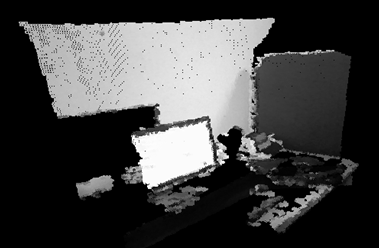
\includegraphics[width=6cm]{images/methodology/FVR/capFrameA}
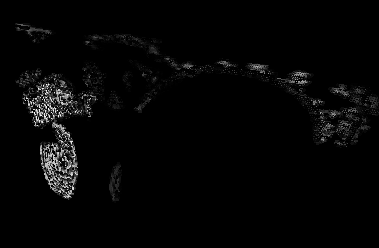
\includegraphics[width=6cm]{images/methodology/FVR/capFrameLogPolar}
\caption{Left: Captured 3D frame, Right: Log-Polar Transform of the captured 3D frame}
\label{fig:LogPolarTransform3DExample}
\end{figure}

The output x coordinate, $X_{log-spherical}$ in the log-spherical transform centres the input x and y coordinates about the centre of the volume and uses the atan trigonometric function to obtain the angle in degrees the point is around the y-axis. This is scaled to the full size of the volume via scalar $\frac{N}{360}$. The result is that data at different angles about the y-axis are linearly grouped by their particular angle along the output x-axis. The output y-coordinate $Y_{log-spherical}$ is also centred about the volume centre and is put through the cosine function. This gives the angle in degrees about the secondary axis (x rotational axis). The degree between 0 and 180 is then mapped to the range $[0-N]$ using the scalar $\frac{N}{180}$. The y coordinate can be directly passed to the cosine function because it is known that the x rotational angle can be computed as the cosine function of the dot product between the input point, $[x,y,z]^T$ and the vertical axis $[0,1,0]^T$ which results in $x \times 0 + y \times 1 + z \times 0 = y$. \\

The output z coordinate, $Z_{log-spherical}$ encompasses the scale information of the input coordinate. First, the distance between the input coordinate and the centre of the volume is computed. This is placed through a log function, the log function compresses the distance such that any scaling relationship between distances becomes a relationship of addition, or in this case volume translation along the z-axis. This is then mapped using the scalar $\frac{N}{log\left(\frac{N}{2.56}\right)}$. This mapping is used so that scales within the range $[2.56^{-1}, 2.56]$ may be registered. Increasing this range too much results in decreased precision and possibly a decrease in accuracy or an inconclusive registration result. \\


\begin{equation} \label{eqn:Log_Spherical}
\begin{split}
X_{log-spherical} & = \frac{atan\left(
\left( x-\frac{N}{2} \right) \times
\left(y-\frac{N}{2}\right)^{-1}
\right)N}{360}\\
Y_{log-spherical} & = \frac{acos\left(
y-\frac{N}{2}
\right)N}
{180} \\
Z_{log-spherical} & =\frac{log\left(
\sqrt{\left(x-\frac{N}{2}\right)^2+\left(y-\frac{N}{2}\right)^2+\left(z-\frac{N}{2}\right)^2}
\right)N}{log\left( \frac{N}{2.56} \right)} \\
\end{split}
\end{equation}

The log-spherical transforms of $M'_1$ and $M'_2$ are then related by translation. The translation relationship describes the camera rotation and the scale factor separating both of the original frames. The exact translational differences can easily be recovered using phase correlation. The resulting peak location from the phase-correlation procedure, $(x_{M'},y_{M'},z_{M'}) = PhaseCorrelation(M'_1, M'_2)$ is used to estimate the rotation and the scale. The phase correlation surface of these two volumes is often very noisy. It is usually noisier than phase correlating data from the spatial domain. Filtering techniques may be used to alleviate this issue. If multiple peaks are detected, the rotation and scale may also be tested for each candidate peak. The rotation $\theta$ and scale factor $\varphi$ separating the two original frames, $V_1$ and $V_2$ can then be computed using the peak values on the phase correlation surface, $(x_{M'},y_{M'},z_{M'})$. The functions to compute $\theta$ and $\varphi$ are given in equation \ref{eqn:ROTATIONSCALEFROMXM}. \\
 
\begin{equation} \label{eqn:ROTATIONSCALEFROMXM}
\begin{split}
\theta & = \frac{-360x_{M'}}{N}\\
\varphi & = e^{
-\left(
2.56^{-1}N
\right)z_{M'}N^{-1}
}
\end{split}
\end{equation}

The $x_{M'}$ coordinate is mapped to a unit number in the range $[0,1]$ and is scaled by $-360$ resulting in $\theta$, the angle of rotation which may be used to align the frames. The $z_{M'}$ coordinate is also mapped to a unit number, it is then scaled by $\frac{N}{256}$ to align the result prior to inverting the log function effects. The value is negated also, this gives the relationship relative to frame 1 rather than frame 2. Finally, the log function is reversed using the exponential function. The resulting rotation matrix may be formed as in equation \ref{eqn:RoteRegMatrix}. This conjuncted matrix first transforms the centre of the volume to the origin and then rotates it by $\theta$, then transforms it back to the centre of the volume. \\

\begin{equation} \label{eqn:RoteRegMatrix}
\left[
\begin{array}{cccc}
1 & 0 & 0 & \frac{N}{2} \\
0 & 1 & 0 & \frac{N}{2} \\
0 & 0 & 1 & \frac{N}{2} \\
0 & 0 & 0 & 1 \\
\end{array}
\right] \times
\left[
\begin{array}{cccc}
cos(\theta) & 0 & sin(\theta) & 0 \\
0 & 1 & 0 & 0 \\
-sin(\theta) & 0 & cos(\theta) & 0 \\
0 & 0 & 0 & 1 \\
\end{array}
\right] \times
\left[
\begin{array}{cccc}
1 & 0 & 0 & -\frac{N}{2} \\
0 & 1 & 0 & -\frac{N}{2} \\
0 & 0 & 1 & -\frac{N}{2} \\
0 & 0 & 0 & 1 \\
\end{array}
\right]
\end{equation}

The resulting scaling matrix is formed similarly (equation \ref{eqn:ScaleRegMatrix}) by transforming the volume centre to the origin, scaling the geometry and then transforming the data back to the centre of the volume. The resulting matrix to un-do both the scale and rotational effects of the camera movement can therefore be computed as the scale matrix multiplied by the rotational matrix, $SR_{matrix} = S_{matrix} \times R_{matrix}$. \\

\begin{equation} \label{eqn:ScaleRegMatrix}
\left[
\begin{array}{cccc}
1 & 0 & 0 & \frac{N}{2} \\
0 & 1 & 0 & \frac{N}{2} \\
0 & 0 & 1 & \frac{N}{2} \\
0 & 0 & 0 & 1 \\
\end{array}
\right] \times
\left[
\begin{array}{cccc}
\varphi & 0 & 0 & 0 \\
0 & \varphi & 0 & 0 \\
0 & 0 & \varphi & 0 \\
0 & 0 & 0 & 1 \\
\end{array}
\right] \times
\left[
\begin{array}{cccc}
1 & 0 & 0 & -\frac{N}{2} \\
0 & 1 & 0 & -\frac{N}{2} \\
0 & 0 & 1 & -\frac{N}{2} \\
0 & 0 & 0 & 1 \\
\end{array}
\right]
\end{equation}

If frame 1, $V_1$ is then transformed by the scale-rotation matrix $SR_{matrix}$, the resulting volumes are separated only by translation. The translation matrix separating them may then be computed using phase correlation. The result of this procedure is that the rotation factor $\theta$, the scale factor $\varphi$ and the translation factors $x$, $y$ and $z$ have all been recovered. Given the translation matrix, $T$, formed by the translation factors $x$, $y$ \& $z$, the full registration matrix aligning frames $V_1$ and $V_2$ may be computed as, $M_{T,\varphi,\theta} = T \times SR_{matrix}$. $M_{T,\varphi,\theta}$. This matrix can be used to align frame 1 to frame 2 prior to integration. Alternatively frame 2 may be aligned with frame 1 by transforming it by $M_{T,\varphi,\theta}^{-1}$. \\

The camera pose relationship between frame 1 and frame 2 is also now known. Given the camera coordinate axes in frame 1, $Forward \in R^3$, $Right \in R^3$, $Up \in R^3$, the coordinate space for the camera in frame 2 may be computed by adjusting these axes by the registration matrix $M_{T,\varphi,\theta}$. Once the camera pose is known, the camera may be tracked by repeating the process between successive frames. The resulting dense 3D data may then be integrated to create the complete 3D reconstruction. Alternatively, the dense 3D data may be projected and integrated directly resulting in the output 3D reconstruction. \\

\subsubsection{Conclusion}

In this section, the volume registration method is applied to 3D pose estimation. In the next section, the method is extended into a full 3D reconstruction algorithm. Experiments in sections \ref{Sec:FVRSOTA} and \ref{Sec:CamTransTrackExp}
show that this method is capable of accurately reconstructing scenes using different sensors whilst being robust to noise. 
